\documentclass{article}
\usepackage[margin=1in, top = .8in, left=.8in]{geometry}
\usepackage{comment}
\usepackage{amsmath, amssymb}
\usepackage{framed}
\usepackage{enumerate}
\usepackage{comment}
\usepackage{tikz,pgfplots}
\usepgfplotslibrary{fillbetween}
\pgfplotsset{compat=1.15}
\usepackage[hyphens]{url}

\begin{document}

\begin{center}
    \large \textbf{Homework 6}
\end{center}
    %\item[\textbf{Week 6}]
        \begin{itemize}
            %\item Sync (week 5):
            \item Part 1
                \begin{enumerate}
                    \item Consider the function
                    $$G(x) = \int_0^x 4-t^2+5t\,dt$$
                    \begin{enumerate}
                        \item On what intervals is $G(x)$ increasing?
                        \item At what value of $x$ is $G(x)$ increasing the fastest?
                        \item At what values of $x$ is $G(x)=0$?
                        \item What is the absolute maximum value of $G(x)$ on the interval $x \in [0,\infty)$? Give complete reasoning.
                    \end{enumerate}
                     \item The peak of Boulder, Colorado's epic rainstorm of 2013 occurred between 4 p.m., September 12 and 4 a.ma, September 13. During those 12 hours the rate of rainfall can be modelled by $\displaystyle r(t)=\frac{240e^{2t/3}}{\left( 60+e^{2t/3} \right)^2}$ in inches per hour, where $t=0$ represents 4 p.m. on September 12.

\begin{center}
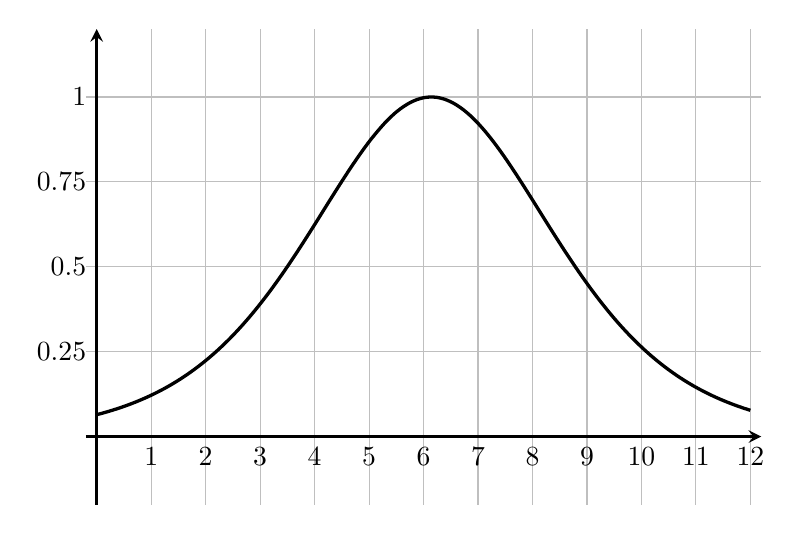
\begin{tikzpicture}
\begin{axis}[
   	xmin=-.2, xmax=12.2,
	ymin=-.2, ymax=1.2,
	major tick length={0},
	line width=1pt,
 	axis lines=center, height=3 in, width=4 in, grid=major, ytick={0,.25,...,1}, xtick={0,1,...,12},
	]
	\addplot [smooth, very thick, samples=99, domain=0:12] {(240*e^(2*x/3))*(60+e^(2*x/3))^(-2)};
\end{axis}
\end{tikzpicture}
\end{center}

Let $\displaystyle R(x)=\int_0^x \frac{240e^{2t/3}}{\left( 60+e^{2t/3} \right)^2} \,dt$.
\begin{enumerate}


%\vfill
\item Use technology to calculate $R(4)$ and $R(12)$. What do these numbers represent? Include units.
%\sol{At $R(4) \approx 1$. This represents the total number of inches of rain that have fallen between 4pm, Sept 12, and 4 hours later, at 8pm, Sept 12.}
%\sol{At $R(12) \approx 5.78326$. This represents the total number of inches of rain that have fallen between between 4pm, Sept 12, and 12 hours later, at 4am, Sept 13.}
%\vfill
%\item What does $R(x)$ represent?
%\sol{The amount of rain that has fallen between 4pm, Sept 12 and $x$ hours later.}
%\vfill
\item Where is $R(x)$ increasing?
\item Where is $R(x)$ changing the fastest?
%\sol{At $x=6$.}
%\vfill
\item Use the graph to estimate $R'(6)$ and $R''(6)$.
\end{enumerate}
                    \item The function $H(x)$ is defined below. Find $H'(2)$.
                    $$H(x) = \int_{-4}^{x} t^2e^{-t^2}\,dt$$
                    \item Compute
                    $$\frac{d}{dx} \int_{\ln{x}}^{e^{x^2}} \frac{t^3}{t^2+1}\,dt$$
                    \item Let $p(x)$ be a constant $c$ on the interval $[0,2]$, and $0$ elsewhere.
                    \begin{enumerate}
                        \item If $p(x)$ is a probability density function, then what is the value of the constant $c$?
                        \item Find a formula for the cumulative distribution function $\displaystyle P(x)=\int_0^x p(t)\,dt$. Write the answer as a piecewise function. 
                        \item Graph $P(x)$.
                        
                    \end{enumerate}
                \item The following is a graph of a function $g(x)$, which is a probability density function. The function $g(x)$ is $0$ on $(-\infty,0]$ and $[4,\infty)$.
                        \begin{center}
        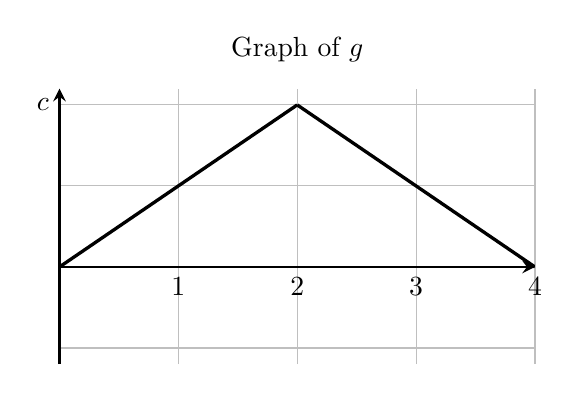
\begin{tikzpicture}
        \begin{axis}[
   	        xmin=0, xmax=4,
	        ymin=-1.2, ymax=2.2,
	        major tick length={0},
	        line width=1pt,
	        %xticks = {0,1,2,3,4},
 	        axis lines=center, height=2 in, width=3 in, grid=major,
 	        title = Graph of $g$,
 	        yticklabels = {, , ,,$c$}
	        ]
	    \addplot [black, smooth, very thick] plot coordinates {(0,0)(2,2)};
	    \addplot [black, smooth, very thick] plot coordinates {(2,2)(4,0)};

        \end{axis}
        \end{tikzpicture}
        \end{center}
                \begin{enumerate}
                    \item Find the value of $c$ needed to make $g$ a probability density function. thus determining the scale on the $y$-axis of the graph.
                    \item Write the formula for the cumulative distribution function as a piecewise function.
                    \item Graph the cumulative distribution function.
                    \item Find the probability that a number with this distribution lies between $3$ and $4$.
                \end{enumerate} 
                \end{enumerate}
            %\item Async (Week 6):
            \item Part 2
                \begin{enumerate}
                    \item Evaluate the following limits.
                        \begin{enumerate}
                            \item $\displaystyle \lim_{x\rightarrow \infty} \frac{\ln(\frac{1}{x})}{e^x}$
                            \item $\displaystyle \lim_{x\rightarrow \infty} \frac{\sqrt{x^2+6x}}{x}$
                            \item $\displaystyle\lim_{x \rightarrow 0} \frac{1}{x\ln{x}}$
                            \item $\displaystyle \lim_{x \rightarrow 1} \left(\frac{x}{x-1} - \frac{1}{\ln{x}}\right)$
                            \item $\displaystyle \lim_{x\rightarrow \infty} (8+x^2)^{3/x}$  (HINT: In order to see this as $``\frac{\infty}{\infty}"$, let $y=(x^2+8)^{3/x}$ and consider $\ln(y)$).
                        \end{enumerate}
                    \item Two of the following integrals can be evaluated in closed form. Determine which two and evaluate them. 
                        \begin{itemize}
                            \item $\displaystyle \int_0^\infty e^{-x^2}\,dx$
                            \item $\displaystyle \int_0^\infty xe^{-x^2}\,dx$
                            \item $\displaystyle \int_0^\infty x^2e^{-x^2}\,dx$
                            \item $\displaystyle \int_0^\infty x^3e^{-x^2}\,dx$
                        \end{itemize}
                    \item Suppose $f(x)=\begin{cases} k & a\leq x\leq b \\ 0 & \textnormal{ otherwise} \end{cases}$.  Determine the value of $k$ so that $\displaystyle \int_{-\infty}^{+\infty} f(x)\ dx =1$.  Then determine the value of $\displaystyle \int_{-\infty}^{+\infty} xf(x)\ dx$.
                    \item Evaluate the integral.  If it is convergent, then determine its value.  Otherwise, show that it is divergent.
                        \begin{enumerate}
                            \item $\displaystyle \int_9^\infty \frac{5x}{x^2\sqrt{x}}\,dx$
                            \item $\displaystyle \int_9^\infty \frac{5x}{x\sqrt{x}}\,dx$
                            \item $\displaystyle \int_1^\infty e^{-7x}\, dx$
                            \item $\displaystyle \int_{0}^1 \frac{x^2}{x^3-1}\, dx$
                            \item $\displaystyle \int_{0}^2 \frac {3}{(x-1)^{2/3}}\, dx$
                            \item $\displaystyle \int_0^\infty \frac{1}{x\ln{x}}\,dx$
                        \end{enumerate}
                    \item Determine if the integral converges or diverges.
                        \begin{enumerate}
                            \item $\displaystyle \int_3^\infty \frac{2x}{4x^2+7}\, dx$
                            \item $\displaystyle \int_1^\infty \frac{dx}{x^3e^x}$
                            \item $\displaystyle \int_1^\infty \frac{\ln x}{x^3}\, dx$
                            \item $\displaystyle \int_1^\infty \frac{\sin^2 x}{4x^5+x}\, dx$
                            \item $\displaystyle \int_1^\infty \frac{dx}{2^x-x}$
                        \end{enumerate}
                \end{enumerate}
        \end{itemize}

\end{document}